\section{Recovery: Basic Concepts, ARIES}

\paragraph{WAL \& the Log}

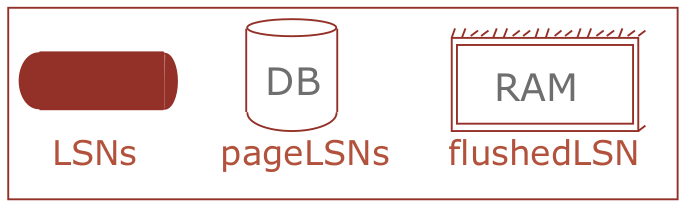
\includegraphics[scale=0.2]{graphics/log-components.png}

\begin{itemize}
\item Each log record has a unique Log Sequence Number (LSN)
  \begin{itemize}
  \item LSNs always increasing
  \end{itemize}

\item Each data page contains a pageLSN
  \begin{itemize}
  \item The LSN of the most recent log record for an update
    to that page
  \end{itemize}

\item System keeps track of flushedLSN
  \begin{itemize}
  \item The max LSN flushed so far
  \end{itemize}

\item WAL: Before a page is written
  \begin{itemize}
  \item pageLSN <= flushedLSN
  \end{itemize}
\end{itemize}

\paragraph{Log Records}
\begin{minipage}{0.3\textwidth}
  \begin{itemize}
  \item Possible log record types
    \begin{itemize}
    \item Update
    \item Commit
    \item Abort
    \item End (signifies end of commit or abort)
    \item Compensation Log Records (CLRs) \\
      → for UNDO actions
    \end{itemize}
  \end{itemize}
\end{minipage}%
\begin{minipage}{0.2\textwidth}
  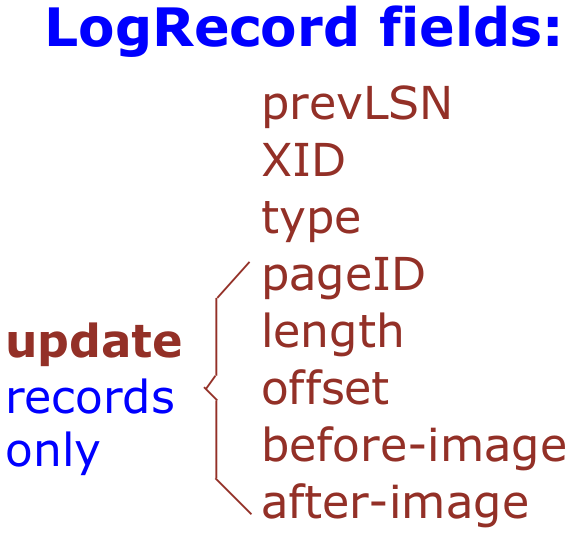
\includegraphics[scale=0.13]{graphics/log-record-fields.png}
\end{minipage}


\paragraph{Other Log-Related State}
\begin{itemize}
\item Transaction Table
  \begin{itemize}
  \item One entry per active Xact
  \item Contains XID, Status (running/commited/aborted) and lastLSN
  \end{itemize}

\item Dirty Page Table:
  \begin{itemize}
  \item One entry per dirty page in buffer pool
  \item Contains recLSN -- the LSN of the log record which first
    caused the page to be dirty
  \end{itemize}
\end{itemize}


\paragraph{Normal Execution of an Xact}
\begin{itemize}
\item Series of reads \&writes, followed by commit or abort
  \begin{itemize}
  \item We will assume that write is atomic on disk \\
    (In practice, additional details to deal with non-atomic writes)
  \end{itemize}

\item Strict 2PL → concurrency is correctly handled

\item STEAL, NO-FORCE buffer management with Write-Ahead Logging
\end{itemize}

\paragraph{The Big Picture: What's Stored Where}

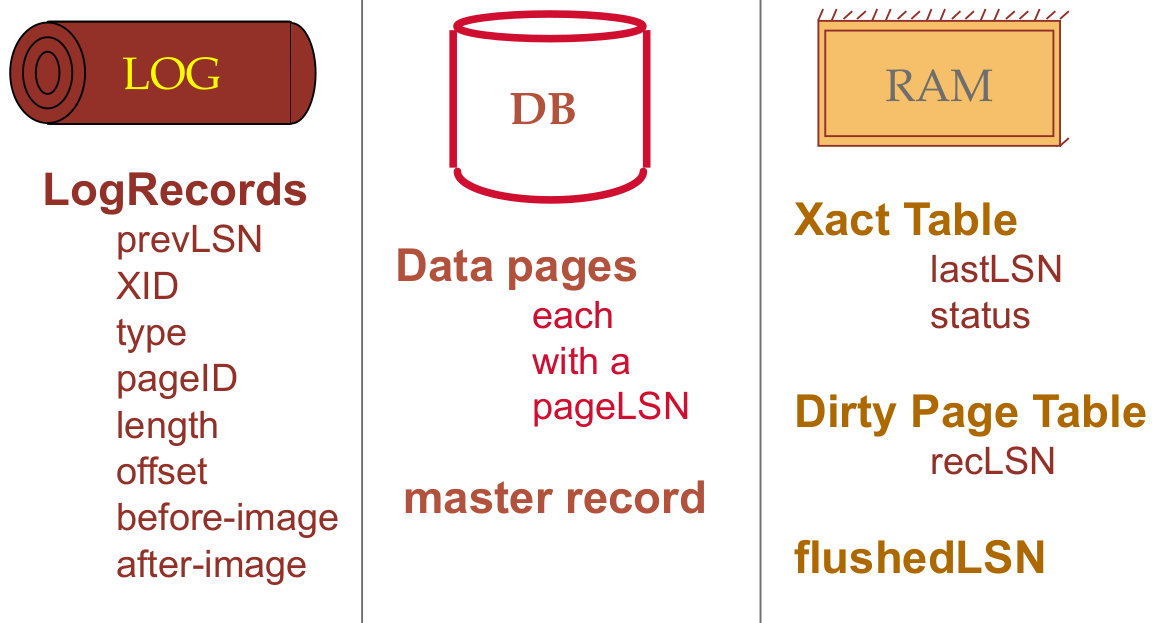
\includegraphics[scale=0.15]{graphics/logging-big-picture.png}


\paragraph{Checkpointing}
\begin{itemize}
\item Periodically, the DBMS creates a \textbf{checkpoint}, to minimize
  the time taken to recover in the event of a system crash.
\item Checkpoint: Write to log
  \begin{itemize}
  \item begin\_checkpoint record: indicates when checkpoint began
  \item end\_checkpoint record: contains current Xact table and
    dirty page table. \\
    This is a 'fuzzy checkpoint':
    \begin{itemize}
    \item Other Xacts continue to run; so these tables accurate only
      as of the time of the begin\_checkpoint record
    \item \textbf{No attempt to force dirty pages to disk};
      effectiveness of checkpoint limited by oldest unwritten change to
      a dirty page, {\color{red} minDirtyPagesLSN}
    \item use \textbf{background process} to flush dirty pages
      to disk!
    \end{itemize}

  \item Store LSN of checkpoint record in a safe place
    (\textbf{master} record)
  \end{itemize}
\end{itemize}

\paragraph{Transaction Commit}
\begin{itemize}
\item Write commit record to log
\item All log records up to Xact's lastLSN are flushed
  \begin{itemize}
  \item Guarantees that flushedLSN >= lastLSN
  \item Note that log flushes are sequential, synchronous
    writes to disk
  \item Many log records per log page
  \end{itemize}

\item Commit() returns
\item Write end record to log
\end{itemize}


\paragraph{Simple Transaction Abort}
\begin{itemize}
\item For now, consider an explicit abort of a Xact
  \begin{itemize}
  \item No crash involved
  \end{itemize}

\item We want to ``play back'' the log in reverse order,
  UNDOing updates
  \begin{itemize}
  \item Get lastLSN of Xact from Xact table
  \item Can follow chain of log records backward via the prevLSN
    field
  \end{itemize}

\item Before starting UNDO, write an Abort log record.
  \begin{itemize}
  \item For recovering from crash during UNDO!
  \end{itemize}
\end{itemize}

\begin{itemize}
\item To perform UNDO, must have a lock on data!
  \begin{itemize}
  \item Strict 2PL enforces this
  \end{itemize}

\item Before restoring old value of a page, write a CLR:
  \begin{itemize}
  \item You continue logging while you UNDO!!
  \item CLR has one extra field: undonextLSN
    \begin{itemize}
    \item Points to the next LSN to undo (i.e. the prevLSN of record
      we are currently undoing)
    \end{itemize}
  \item CLRs \textbf{never} undone (but they might be Redone when
    repeating history: guarantees Atomicity!)
  \end{itemize}

\item At end of UNDO, write and end log record
\end{itemize}


\paragraph{Example}
\begin{itemize}
\item 10 T1 writes  P5
\item 20 T2 writes P17
\item 30 T1 writes P3
\end{itemize}
\textbf{P3 written to disk (pageLSN for page 3 at this time is 30)}
\begin{itemize}
\item 40 T1 aborts
\item 50 CLR T1 P3 (undonextLSN: 10)
\item 60 CLR T1 P5 (undonextLSN: NULL)
\item 70 End T1
\end{itemize}


\paragraph{Crash Recovery: Big Picture}


\begin{minipage}{0.365\textwidth}
  \begin{itemize}
  \item Start from a checkpoint (found via master record)
  \item Three phases
    \begin{itemize}
    \item Figure out which Xacts committed since checkpoint, \\
      which failed ({\color{blue} Analysis})
    \item {\color{brown} REDO} all actions (Repeat History)
    \item {\color{green} UNDO} effects of failed Xacts
    \end{itemize}
  \end{itemize}
\end{minipage}%
\begin{minipage}{0.2\textwidth}
  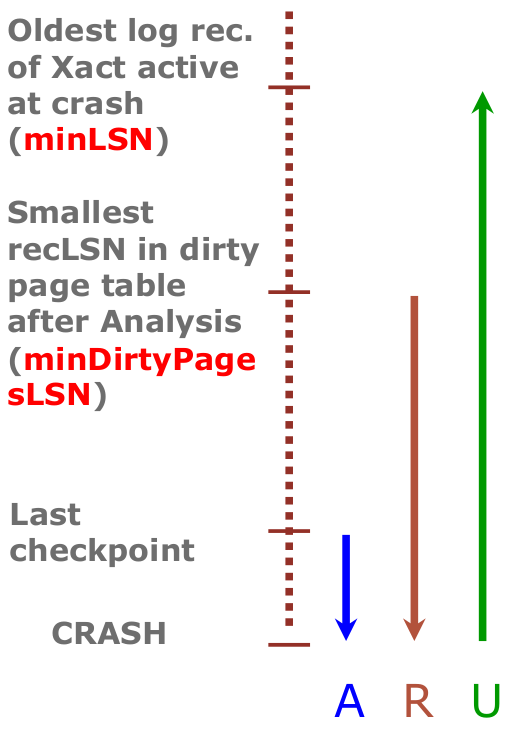
\includegraphics[scale=0.1]{graphics/crash-recovery-phases.png}
\end{minipage}

\paragraph{Recovery: The Analysis Phase}
\begin{itemize}
\item Reconstruct state (Xact table and dirty page table)
  at checkpoint
  \begin{itemize}
  \item via end\_checkpoint record
  \end{itemize}

\item Scan log forward from checkpoint
  \begin{itemize}
  \item End record: Remove Xact from Xact table
  \item Other records: Add Xact to Xact table, set
    lastLSN=LSN, change Xact status on commit
  \item Update record: if P not in Dirty Page Table,
    \begin{itemize}
    \item Add P to Dirty Page Table, set its recLSN=LSN
    \end{itemize}
  \end{itemize}
\end{itemize}


\paragraph{Recovery: The REDO Phase}
\begin{itemize}
\item We repeat History to reconstruct state at crash:
  \begin{itemize}
  \item Reapply all updates (even of aborted Xacts!), redo CLRs
  \end{itemize}

\item Scan forward from log record containing the smallest
  recLSN in Dirty Page Table. For each CLR or update log
  record with LSN, REDO the action unless:
  \begin{itemize}
  \item Affected page is not in the Dirty Page Table, or
  \item Affected page is in Dirty Page Table, but has recLSN > LSN,
    or
  \item pageLSN (in DB) >= LSN
  \end{itemize}

\item To REDO an action:
  \begin{itemize}
  \item Reapply logged action
  \item Set pageLSN to LSN, no additional logging!
  \end{itemize}
\end{itemize}

\paragraph{Recovery: The UNDO Phase}
$\text{ToUndo} = \{lsn | lsn \text{ a lastLSN of a ``loser'' Xact}\}$

\textbf{Loser Transactions:} all transactions active at the time
of the crash. All actions of losers must be undone, and further,
these actions must be undone in the reverse of the order in which
they appear in the log.

\begin{itemize}
\item \textbf{Repeat:}
  \begin{itemize}
  \item Choose largestLSN among ToUndo
  \item If this LSN is a CLR and undonextLSN==NULL
    \begin{itemize}
    \item Write an End record for this Xact
    \end{itemize}

  \item If this LSN is a CLR, and undonextLSN != NULL
    \begin{itemize}
    \item Add undonextLSN to ToUndo
    \end{itemize}

  \item Else this LSN is an update. Undo the update write a CLR,
    add prevLSN to ToUndo
  \end{itemize}
\item \textbf{Until ToUndo is empty}
\end{itemize}

\paragraph{Example Recovery: Notes}
No optimization in terms of removing pages that we know
are clean after a transaction has been aborted, because
in the present of other transactions we cannot be sure
that page is clean.

When undoing a page at it is not yet in the dirty page table
we have to put it there.

Recovery is the same as normal execution (just redoing it
to reconstruct state (Transaction Table and Dirty Page Table).



% LocalWords:  WAL LSN LSNs pageLSN flushedLSN CLRs Xact XID lastLSN
% LocalWords:  recLSN Checkpointing Xacts minDirtyPagesLSN CLR ToUndo
% LocalWords:  undonextLSN Atomicity lsn largestLSN Xact's UNDOing
% LocalWords:  prevLSN
